% Тут используется класс, установленный на сервере Papeeria. На случай, если
% текст понадобится редактировать где-то в другом месте, рядом лежит файл matmex-diploma-custom.cls
% который в момент своего создания был идентичен классу, установленному на сервере.
% Для того, чтобы им воспользоваться, замените matmex-diploma на matmex-diploma-custom
% Если вы работаете исключительно в Papeeria то мы настоятельно рекомендуем пользоваться
% классом matmex-diploma, поскольку он будет автоматически обновляться по мере внесения корректив
%

% По умолчанию используется шрифт 14 размера. Если нужен 12-й шрифт, уберите опцию [14pt]
%\documentclass[14pt]{matmex-diploma}
\documentclass[14pt]{matmex-diploma-custom}

\hyphenation{op-tical net-works semi-conduc-tor con-tract Et-he-re-um}
\hyphenation{пре-по-да-ва-тель сту-дент вы-чис-ли-тель-но}
\newcommand\name[1]{\textsc{#1}}
\newcommand\achtung[1]{{\color{red}#1}}

\usepackage{longtable,booktabs,threeparttablex}
\usepackage{makecell}
\usepackage[export]{adjustbox}
\usepackage{afterpage}


\begin{document}
% Год, город, название университета и факультета предопределены,
% но можно и поменять.
% Если англоязычная титульная страница не нужна, то ее можно просто удалить.
\filltitle{ru}{
    chair              = {Программная инженерия\\ Кафедра системного программирования},
    title              = {Проектирование и реализация среды исполнения смарт-контрактов для блокчейна Hyperledger Iroha},
    % Здесь указывается тип работы. Возможные значения:
    %   coursework - Курсовая работа
    %   diploma - Диплом специалиста
    %   master - Диплом магистра
    %   bachelor - Диплом бакалавра
    type               = {bachelor},
    author             = {Тюляндин Иван Владимирович},
    supervisorPosition = {ст. преп.},
    supervisor         = {Кириленко Я. А.},
    consultantPosition   = {программист ООО "Интеллиджей Лабс"\\ к.\,ф.-м.\,н.},
    consultant           = {Березун Д. А.},
    reviewerPosition   = {Генеральный директор ООО «Сорамитсу Лабс»\\},
    reviewer           = {Салахиев К. Р.}
%   university         = {Санкт-Петербургский Государственный Университет},
%   faculty            = {Математико-механический факультет},
%   city               = {Санкт-Петербург},
%   year               = {2013}
}
\filltitle{en}{
    chair              = {Software Engineering},
    title              = {Design and implementation of smart contracts execution environment for Hyperledger Iroha blockchain},
    author             = {Ivan Tyulyandin},
    supervisorPosition = {Senior lecturer},
    supervisor         = {Iakov Kirilenko},
    consultantPosition   = {IntelliJ Labs Co. Ltd developer\\ PhD},
    consultant           = {Daniil Berezun},
    reviewerPosition     = {Soramitsu Labs CEO},
    reviewer             = {Kamil Salakhiev}
    % chairHeadPosition  = {professor},
    % chairHead          = {Christobal Junta},
}
\maketitle
\tableofcontents
% У введения нет номера главы


\section*{Введение}

Скрытые марковские модели~\cite{HMM_wiki}.

\section{Обзор}
В этой главе будут рассмотрены среды исполнения и языки смарт-контрактов, а так же некоторые особенности \name{Hyperledger Iroha}.

\subsection{Языки и среды исполнения смарт-контрактов}
В 1997 году Ник Сабо (Nick Szabo) предложил концепцию смарт-контрактов~\cite{Szabo_SC}.
Смарт-контракт --- это программа, которая описывает взаимодействие участников блокчейн-сети. 
При сравнении с традиционным бумажным контрактом, смарт-контракт имеет однозначную семантику и выполняется автоматически при достижении определенных условий.
Результат выполнения смарт-контракта легко подтверждается, так как он будет записан в историю транзакций блокчейна.
На сегодняшний день существует множество различных языков смарт-контрактов и блокчейнов, которые могут исполнять программы на этих языках.

Смарт-контракт всегда должен завершаться для продолжения работы блокчейн-сети.
Если язык смарт-контрактов Тьюринг-полный, то среда исполнения должна предоставлять механизм, который будет ограничивать тем или иным способом количество операций смарт-контракта.
В случае \name{Ethereum} каждая инструкция стоит определенное количество \emph{газа}, цена которого выражена во внутренней криптовалюте \name{Et\-he\-re\-um}.
В \name{Hyperledger Fabric} имеется ограничение на время выполнения кода смарт-контракта.
Для языка \name{Rholang}~\cite{Rholang}, основанном на \name{Rho-calculus}~\cite{RhoCalculus}, выставляется лимит по количеству применений правил редукции.

Далее будут рассмотрены несколько сред исполнения смарт-кон\-трак\-тов и языки, которые данные среды поддерживают.

\subsubsection{Языки смарт-контрактов}
В этой подглаве рассмотрены языки смарт-контрактов с учетом их парадигм и свойств, таких как Тьюринг-полнота, механизм ограничения выполнения смарт-контракта платформой (на которой смарт-контракт исполняется) и системы типов.

На данный момент существуют языки смарт-контрактов с различным уровнем абстракции. 
\emph{Низкоуровневые языки} (low-level) предназначены для непосредственного выполнения средой исполнения.
Многие концепции, такие как семантика, вычислительная модель, система ограничения выполнения и типизация часто описываются на этом уровне.
Примеры таких языков --- \name{EVM}~\cite{EthereumYellowPaper}, \name{Bitcoin Script}~\cite{BitcoinScript} и \name{Michelson}~\cite{Michelson}.
\emph{Высокоуровневые языки} (high-level), такие как \name{Solidity}~\cite{Solidity}, \name{Flint}~\cite{Flint} и \name{Liquidity}~\cite{liquidity},
упрощают процесс разработки смарт-контрактов за счет повышенной читаемости, наличия более абстрактных синтаксических конструкций и системы типов.
\emph{Промежуточные языки} (intermediate-level) смарт-контрактов являются своего рода компромиссом между высокоуровневыми и низкоуровневыми языками по степени абстракции.
Как правило, они спроектированы для упрощения формальной верификации или статического анализа исходного кода (с учетом вычислительной модели, системы типов, семантики и других формализмов).
\name{Scilla}~\cite{Scilla} является промежуточным языком смарт-контрактов.

В ходе обзора языков смарт-контрактов на конференцию SYRCoSE 2019 была написана обзорная статья \emph{A Survey of Smart Contract Safety and Pro\-gram\-ming Languages}, которая будет опубликована в Proceedings of ISP RAS.
Ниже приведена сводная таблица по языкам смарт-кон\-трак\-тов и их свойствам из данной статьи.
В ней приведены следующие характеристики языков смарт-контрактов: название, уровень абстракции, текущее состояние разработки, проект (для которого язык предназначен), парадигма, способ ограничения выполнения смарт-контракта целевой платформой и Тьюринг-полнота соответственно. 


\begin{ThreePartTable}
\renewcommand\TPTminimum{\textwidth}
% Arrange for "longtable" to take up full width of text block
\setlength\LTleft{0pt}
\setlength\LTright{0pt}
\setlength\tabcolsep{0pt}
%\begin{TableNotes}
%\end{TableNotes}
\fontsize{11}{12}\selectfont
\begin{longtable}{  l @{\extracolsep{\fill}} *{6}{c} }
\toprule
    Language & Level & Current & Project
    & Paradigm /& Metering & Turing\\ 
    & & state & & influence & & completeness\\
\midrule
\endhead

\midrule[\heavyrulewidth]
\multicolumn{7}{r}{\textit{продолжение}}\\
\endfoot  

\midrule[\heavyrulewidth]
%\insertTableNotes  % tell LaTeX where to insert the table-related notes
\endlastfoot

Bamboo & high-level & alpha & Ethereum & functional 
& \centering {gas system} & yes\\
& & (experimental) & & & &\\
\addlinespace

Bitcoin & low-level & under & Bitcoin & stack-based, 
& script size & no\\
Script & & development & & reverse-polish & &\\
\addlinespace

Chain-& high-level & stable & Hyperledger & general purpose & timeout & yes\\
code & & & Fabric & languages & &\\
\addlinespace

EOSIO & high-level& stable & {EOS.IO} & object-oriented, & bound & yes\\
& & & & statically typed & system &\\    
\addlinespace

EVM & low-level& stable & Ethereum & stack-based & \centering gas system & yes\\
bytecode & & & & & &\\
\addlinespace

Flint & high-level & alpha & Ethereum & type safe, & {\centering gas system} & yes\\
& & & & contract-oriented& &\\
\addlinespace

IELE & low-level & prototype & Ethereum & register- & gas system & yes\\
& & & & based & &\\
\addlinespace

Ivy & high-level& prototype & Bitcoin & imperative & gas system & no\\
& & (experimental) & & & & \\
\addlinespace

Liquidity & high-level & under & Tezos & fully-typed, & gas system & yes\\
& & development & & functional & & \\
\addlinespace

LLL & intermediate-& under & Ethereum & stack-based & gas system & yes\\
& level & development & & & & \\
\addlinespace

Logikon & high-level & experimental & Ethereum & logical- & gas system & yes\\
& & & & functional & & \\
\addlinespace

Michelson & low-level & under & Tezos & stack-based, & gas system & yes\\
& & development & & strongly typed & & \\
\addlinespace

Plutus & high-level & under & Cardano & functional & gas system & yes\\
(PlutusCore) & (low-level) & development & & & & \\
\addlinespace

Rholang & high-level& under & RChain & functional & rule reduction & yes\\
& & development & & & system & \\
\addlinespace

Scilla & intermediate-& under & Zilliqa & functional & gas system & no\\
& level & development & & & & \\
\addlinespace

Simplicity & low-level & under & Bitcoin & functional, typed, & Bit Machine & no \\
& & development & & combinator-based & & \\
\addlinespace

Solidity & high-level & stable & Ethereum & statically typed, & gas system & yes\\
& & & & object-oriented & & \\
\addlinespace

SolidityX & high-level & beta & Ethereum & secure- & gas system & yes\\
& & & & oriented & & \\
\addlinespace

Vyper & high-level & beta & Ethereum & imperative & gas system & no\\
& & & & & & \\
\addlinespace

Yul & intermediate-& under & Ethereum & object-oriented & gas system & yes \\
& level & development & & & & \\
\addlinespace

\end{longtable}   
\end{ThreePartTable}

Было выявлено, что \name{Ethereum} является наиболее популярной платформой для работы со смарт-контрактами.
Экосистема данного блокчейна развита --- существует множество языков с различными подходами, сред разработки и статических анализаторов.
Аналогичной экосистемы нет ни у одного из всех рассмотренных блокчейнов.

\subsubsection{\name{Ethereum Virtual Machine}}
% https://habr.com/ru/post/340928/
\name{Ethereum Virtual Machine} (сокращенно \name{EVM}) --- Тьюринг-полная виртуальная стековая машина блокчейна \name{Ethereum}.
Смарт-контракты для этой платформы написаны на байткоде~\cite{EthereumYellowPaper}.
Под эту среду исполнения смарт-контрактов существует множество языков ~\cite{Bamboo, Flint, IELE, Logikon, Solidity, SolidityX, Vyper, LLL, Yul}, которые компилируются в байткод \name{EVM}.

Есть два участка памяти, куда \name{EVM} может записывать значения во время выполнения кода смарт-контракта --- \emph{memory} и \emph{storage}.
Memory является временным хранилищем данных, необходимым для записи промежуточных значений. 
Можно провести аналогию, что memory для \name{EVM} --- это как оперативная память для компьютера.
Ячейки memory адресуются от 0 до $2^{256} - 1$ (по размеру машинного слова \name{EVM} в 256 битов) и содержат байт информации.
Storage представляет из себя хранилище пар вида ключ-значение, которые описывают текущее состояние переменных смарт-контракта.
В отличие от memory, данные storage записываются в блокчейн.
Размер storage равен $2^{256}$ ячеек, каждая из них хранит машинное слово.

Аккаунты в блокчейн сети \name{Ethereum} бывают двух видов: \emph{пользовательские} и \emph{контракты}.
Аккаунты-контракты содержат код, который может быть вызван пользовательским аккаунтом или кодом другого контракта.

\subsubsection{\name{Hyperledger Burrow}}
\name{Hyperledger Burrow} --- \name{EVM} с правами доступа, проект \name{Hy\-per\-led\-ger Fo\-un\-da\-ti\-on}.

\subsection{\name{Hyperledger Iroha}}
\subsubsection{Общие сведения о \name{Hyperledger Iroha}}
Транзакции формируются с помощью набора специальных команд.

\subsubsection{Валидация транзакции}
Прежде чем принять транзакцию, всем участникам сети нужно подтвердить её корректность.
Есть два этапа валидации --- \emph{stateless} и \emph{sta\-te\-ful}.
Транзакция должна быть сформирована согласно некоторым правилам.
Во время stateless валидации контролируется соответствие этим правилам.
Далее проводится stateful валидация. 
На этом этапе проверяется выполнимость отправленной транзакции (например, права доступа или наличие активов). 







\section{Взаимодействие среды исполнения смарт-кон\-трак\-тов с \name{Hy\-per\-led\-ger Iro\-ha}}
В этой главе будет рассмотрена схема взаимодействия среды исполнения смарт-контрактов и программный интерфейс, который эту схему реализует.
\subsection{Схема взаимодействия}
\label{Interaction}
\begin{figure}[h]
    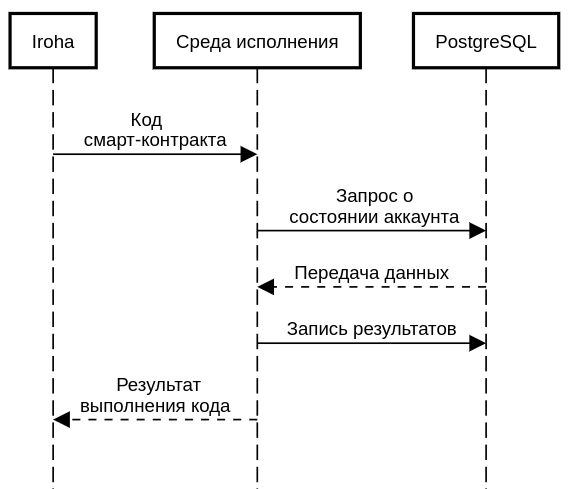
\includegraphics[width=\columnwidth]{interaction.png}
	\caption{Диаграмма последовательности взаимодействия}
	\label {interaction}
\end{figure}
Для создания инфраструктуры для среды исполнения смарт-кон\-трак\-тов необходимо разработать схему взаимодействия этой среды и блокчейна \name{Hy\-per\-led\-ger Iro\-ha}.
Среда исполнения должна уметь получать и записывать данные в блокчейн.

На диаграмме \ref{interaction} показано взаимодействие среды исполнения с \name{Hy\-per\-led\-ger Iro\-ha} и локальной базой данных \name{PostgreSQL}, в которой хранится история транзакций, права доступа и информация о пользователях.
Среда исполнения принимает на вход код смарт-контракта и начинает его выполнение.
Для того, чтобы получать и записывать актуальное состояние переменных смарт-контракта, среда исполнения обращается к базе данных.
Запросы выполняются по необходимости.

\subsection{Реализация интерфейса взаимодействия}
Пользователи формируют транзакции с помощью специального набора команд.
Для работы с командами в коде используется паттерн <<фабричный метод>>.
Для того, чтобы участники могли сохранять и выполнять код смарт-контракта, была добавлена новая команда \emph{Add\-Smart\-Con\-tract}.
Она содержит в себе данные, необходимые для вызова среды исполнения.
То, что будет передано, зависит от конкретной среды исполнения.
Для передачи транзакций и записи в блокчейн используются библиотеки \name{Protobuf} и \name{RapidJSON}, поэтому нужно уметь переводить данные, содержащиеся в AddSmartContract (как и в любой другой команде), в форматы \name{Protocol Buffers} и \name{JSON} и обратно во внутреннее представление.

Перед тем, как транзакция будет записана в истории блокчейна, все участники сети должны провести stateless и stafeful валидацию всех команд внутри этой транзакции.
Для AddSmartContract stateless валидация может содержать различные проверки кода, например на синтаксическую корректность.
Во время stateful валидации участник сети обязан выполнить код и получить новое состояние блокчейна, чтобы в дальнейшем во время работы алгоритма консенсуса все участники договорились, принимать это новое состояние или нет.
\section{Внедрение среды исполнения смарт-кон\-трак\-тов}
В этой главе описаны аргументы для выбора среды исполнения и реализация взаимодействия этой среды с блокчейном \name{Hyperledger Iroha}.

\subsection{Выбор среды исполнения}
Сред исполнения смарт-контрактов огромное количество, необходимо выбрать одну из них.
Была выбрана виртуальная машина из проекта \name{Hyperledger Burrow}, так как она обладает следующими преимуществами: 1) выполнение байт-кода \name{EVM}; 2) наличие программного интерфейса для взаимодействия; 3) проект поддерживается \name{Hy\-per\-led\-ger}; 4) есть примеры интеграции с другими проектами \name{Hy\-per\-led\-ger Fabric}~\cite{HLFabricEVM} и \name{Hyperledger Sawtooth}~\cite{HLSeth}.
Так как \name{Ethereum} де-факто является самой популярной платформой для работы со смарт-контрактами, программистам будет проще адаптироваться к разработке смарт-контрактов для \name{Hy\-per\-led\-ger Iro\-ha}.
Наличие программного интерфейса упрощает имплементацию схемы взаимодействия, описанной в подглаве~\ref{Interaction}.
Важную роль играет принадлежность к \name{Hy\-per\-led\-ger} --- при возникновении проблем и вопросов на этапе интеграции виртуальной машины можно обратиться к сообществу разработчиков указанных ранее проектов.

\subsection{Взаимодействие среды исполнения смарт-кон\-трак\-тов с \name{Hy\-per\-led\-ger Iro\-ha}}
В данной подглаве описано взаимодействие виртуальной машины \name{Hyperledger Burrow} с \name{Hyperledger Iroha}.


\section{Тестирование}
В ходе работы в проект были добавлены два компонента --- интерфейс для взаимодействия со средой исполнения смарт-контрактов (команда AddSmartContract) и виртуальная машина из проекта \name{Hy\-per\-led\-ger Bur\-row}.
Нужно протестировать команду AddSmartContract и реализацию программного интерфейса, необходимого для корректной работы виртуальной машины.
В проекте \name{Hyperledger Iroha} существует инструмент тестирования \name{ITF} (Integration Test Framework), основанный на библиотеке \name{GTest}.
Он позволяет настроить блокчейн и его историю: сформировать аккаунты пользователей, выставить параметры для алгоритма консенсуса, создать заглушку (содержащую данные для формирования транзакций), провести stateless и stateful валидацию заранее заготовленной транзакции.

Для проверки команды Add\-Smart\-Con\-tract были добавлены модульные тесты, проверяющие операции над данными внутри команды, а именно: сериализация в форматы \name{Protocol Buffers} и \name{JSON} и десериализация из них, а также интеграционные тесты на stateless и stateful валидацию.

Для тестирования реализации программного интерфейса, которого требует виртуальная машина, были разработаны модульные тесты, содержащие вызов различных смарт-контрактов, в том числе и невалидных с точки зрения соответствия байт-коду \name{EVM}.
Внутри них выполняются базовые операции, такие как: создание аккаунта-контракта, присваивание и чтение переменных, вызов функции с параметрами.
Проверялась корректность состояния блокчейна после выполнения одного или нескольких смарт-контрактов в одной транзакции.
\section{Текущие результаты}
В ходе работы были выполнены следующие задачи:
\begin{itemize}
	\item сделан обзор предметной области;
	\item реализованы две версии алгоритма Витерби, одна для определения СММ из раздела~\ref{HMM_Vit}, другая для \name{P7Viterbi};
	\item написаны соответствующие специализаторы;
	\item начат сравнительный анализ.
\end{itemize}


Далее необходимо написать преобразователь между разными 
формализмами СММ и \name{P7Viterbi}.
Затем планируется перейти к сравнению специализаторов 
алгоритма Витерби друг с другом и существующими решениями 
задачи гомологичности \name{HMMer} и \name{CUDAMPF}.



\setmonofont[Mapping=tex-text]{CMU Typewriter Text}
\bibliographystyle{ugost2008ls}
\bibliography{diploma.bib}
\end{document}
